\documentclass[class=article,border=5pt,tikz]{standalone}

\begin{document}
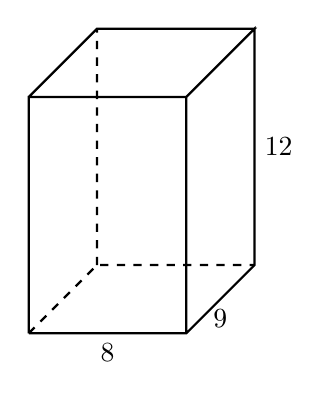
\begin{tikzpicture}[thick,scale=2.5]
\pgfmathsetmacro{\x}{0.8}%
\pgfmathsetmacro{\y}{0.9}%
\pgfmathsetmacro{\z}{1.2}%
\path (0,0,\y) coordinate (A) (\x,0,\y) coordinate (B) (\x,0,0) coordinate (C) (0,0,0)
coordinate (D) (0,\z,\y) coordinate (E) (\x,\z,\y) coordinate (F) (\x,\z,0) coordinate (G)
(0,\z,0) coordinate (H);
\draw (A)-- node[below]{8} (B)-- node[below]{9} (C)--(G) node[midway,right]{12}--(F)--(B) (A)-- (E)--(F)--(G)--(H)--(E);
\draw [dashed,black] (A)--(D)--(C) (D)--(H);
\end{tikzpicture}

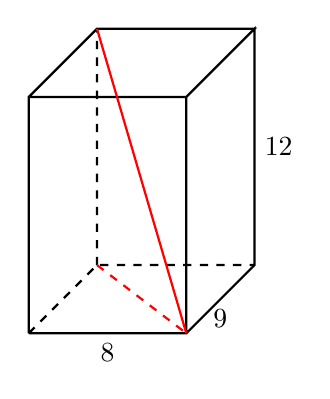
\begin{tikzpicture}[thick,scale=2.5]
\pgfmathsetmacro{\x}{0.8}%
\pgfmathsetmacro{\y}{0.9}%
\pgfmathsetmacro{\z}{1.2}%
\path (0,0,\y) coordinate (A) (\x,0,\y) coordinate (B) (\x,0,0) coordinate (C) (0,0,0)
coordinate (D) (0,\z,\y) coordinate (E) (\x,\z,\y) coordinate (F) (\x,\z,0) coordinate (G)
(0,\z,0) coordinate (H);
\draw (A)-- node[below]{8} (B)-- node[below]{9} (C)--(G) node[midway,right]{12}--(F)--(B) (A)-- (E)--(F)--(G)--(H)--(E);
\draw [dashed,black] (A)--(D)--(C) (D)--(H);
\draw [red] (H) -- (B);
\draw [red,dashed] (D) -- (B);
\end{tikzpicture}
\end{document}


